\subsection{Dữ liệu: Số biến - Đơn biến}
Trực quan hóa GROOVE (Granularity Overview OVErlay) [262] mở rộng trực quan hóa dựa trên pixel bằng cách phủ lên lớp tổng hợp một hoặc nhiều trong 3 phương pháp: (1) lớp phủ theo màu, (2) lớp phủ theo độ mờ hoặc (3) lớp phủ không gian. Các mức tổng hợp là kết quả của các mức độ chi tiết thời gian khác nhau. Các lớp phủ cho phép đọc vi mô và vĩ mô và hướng chuyển động của mắt giữa việc quan sát tổng quan và chi tiết. Với mục đích mình họa, chúng tôi giữ sự hiển thị đơn giản và lượng dữ liệu trực quan không nhiều. Không gian trống xuất hiện do sự bất thường của việc kết hợp các chi tiết tuần và tháng. 
\\ \\
Đầu tiên, các thành phần màu có thể được sử dụng với lớp phủ màu (hình (\ref{fig:f7.5})). Hình này vẽ sơ đồ dữ liệu lưu lượng trong vài tuần. Màu sắc thay đổi từ xanh sang đỏ cho mức thấp hơn hoặc cao hơn trung bình hàng tuần. Hình \ref{fig:f7.5} (a) chỉ thể hiện các giá trị theo tuần. Độ sáng của một ngày cụ thể cao hơn trong trường hợp lưu lượng trong ngày đó cao hơn. Hình \ref{fig:f7.5} (c) chỉ thể hiện giá trị theo ngày. Hình \ref{fig:f7.5} (b) thể hiện lớp phủ màu.
\begin{figure}[H] % places figure environment here   
    \centering % Centers Graphic
    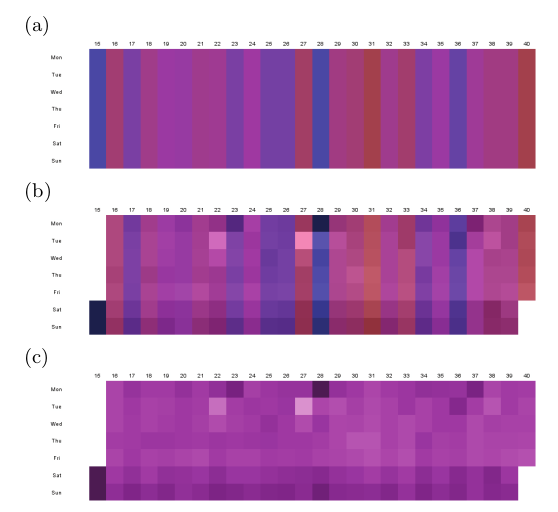
\includegraphics[width=0.8\textwidth]{assets/fig_7_5.png} 
    \caption{Trực quan hóa GROOVE kết hợp đọc chi tiết và tổng quan sử dụng bố cục thông thường dựa trên mức độ chi tiết của thời gian. Ví dụ biểu diễn dữ liệu lấy từ tập Dodgers Loop Sensor [195]. Ở đây lớp phủ màu được sử dụng: (a) Lưu lượng trung bình trên một đoạn đường cao tốc (tuần trong năm từ 15 đến 40) được ánh xạ màu từ xanh qua tím qua đỏ. (c) Lưu lượng trung bình theo ngày được ánh xạ bằng độ sáng. (b) Lớp phủ màu của cả 2 độ chi tiết. (Nguồn: GROOVE modules for TimeBench [339])} % Creates caption underneath graph
    \label{fig:f7.5}
\end{figure}
Thứ hai, lớp phủ mờ (xem Hình (\ref{fig:f7.6})) áp dụng hiệu ứng xen kẽ tương tác giữa hiển thị tổng quan và hiển thị chi tiết. Hình thứ 2 của chúng tôi biểu diễn dữ liệu doanh thu của một cửa hàng trong một năm và sử dụng bố cục đệ quy [223]. Các hàng và cột của các khối lớn hơn được kết hợp với sự sắp xếp các pixel trong các khối cho cấu trúc chi tiết. Các sắp xếp khác nhau có thể được chọn lựa (ví dụ hàng-hàng, sau-trước). Mỗi khối đại diện cho một tháng và các khối được sắp xếp với mỗi hàng cho mỗi quý. Trong các khối, các pixels được sắp xếp với mỗi hàng cho mỗi tuần và mỗi pixel cho một ngày giống như tờ lịch. 
\\ \\
Thứ ba, lớp phủ không gian có thể được sử dụng bằng cách hiển thị các giá trị trung bình như viền bao xung quanh các giá trị chi tiết. Lớp phủ không gian có thể được kết hợp với hai phương pháp khác. Nó cũng có thể được áp dụng sử dụng tương tác bằng cách mở rộng hoặc thu hẹp diện tích theo nhu cầu.
\begin{figure}[H] % places figure environment here   
    \centering % Centers Graphic
    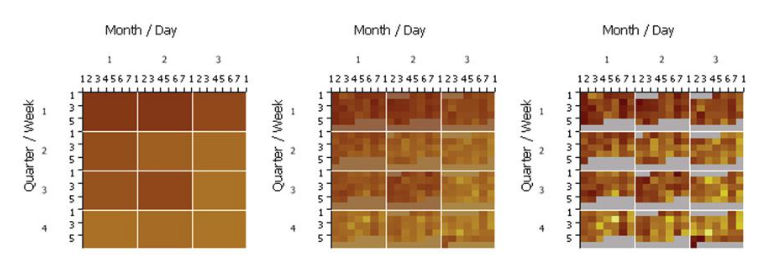
\includegraphics[width=1\textwidth]{assets/fig_7_6.png} 
    \caption{Trực quan hóa GROOVE sử dụng lớp phủ mờ. Dữ liệu được vẽ cho doanh thu hàng ngày của một cửa hàng trong 1 năm; mỗi khối mô tả một tháng: màu đỏ tối thể hiện giá trị thấp và vàng sáng thể hiện giá trị cao. Trong ví dụ này, tổng quan theo tháng được kết hợp với chi tiết ngày sử dụng nhiều độ mờ khác nhau. (Nguồn: GROOVE)} % Creates caption underneath graph
    \label{fig:f7.6}
\end{figure}